%% SW design: PSoC Boundary

\begin{figure}[htbp] \centering
{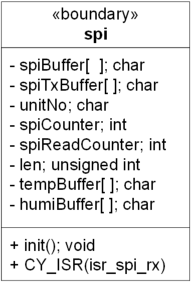
\includegraphics[scale=1.3]{filer/design/Klassediagrammer/sw_psoc_SPIhandler}}
\caption{Klasse spi}
\label{fig:sw_psoc_class_spi}
\end{figure} 

{\centering
\textbf{spi}\par
}
\textbf{Ansvar:} Håndterer kommunikation i mellem Master og Enhed. \

\textbf{Attributter:}
\begin{itemize}
	\item \verb+char spiBuffer[]+ Bruges til modtagede SPI kommandoer fra Master
	\item \verb+char spiTxBuffer[]+ Bruges til afsendelse af SPI kommandoer til Master
	\item \verb+char unitNo+ Enheds nummer til verificering
	\item \verb+int spiCounter+ Tæller til antallet af modtagne data-stykker
	\item \verb+int spiReadCounter+ Tæller til antallet af afsendte data-stykker
	\item \verb+unsigned int len+ Længde til afsendelse af log-data
	\item \verb+char tempBuffer[]+ Midlertidig buffer til konfigurering af parametre
	\item \verb+char humiBuffer[]+ Midlertidig buffer til konfigurering af parametre
\end{itemize}

\verb+void init( ) +\\
\textbf{Parametre:} Ingen. \\
\textbf{Returværdi:} Ingen. \\
\textbf{Beskrivelse:} Starter \verb+SPIS_1+ komponenten, sætter ISR-callback funktionen til \verb+isr_spi_rx+ og nulstiler RX bufferen. \\

\verb+CY_ISR(isr_spi_rx) +\\
\textbf{Parametre:} Ingen. \\
\textbf{Returværdi:} Ingen. \\
\textbf{Beskrivelse:} Læser modtaget data og kalder de aktuelle controller-klasser. \\

\begin{figure}[htbp] \centering
{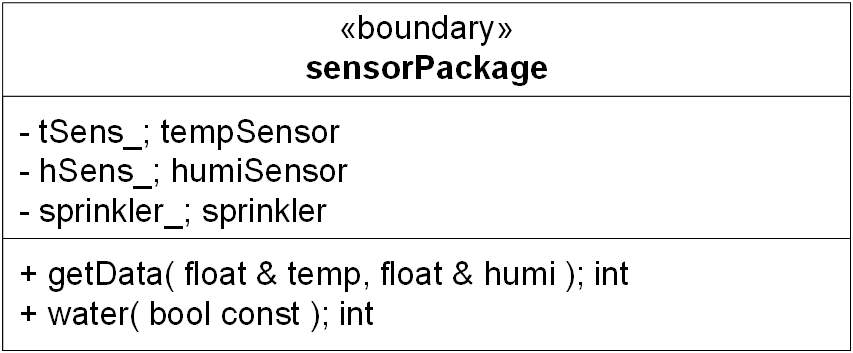
\includegraphics[scale=1.3]{filer/design/Klassediagrammer/sw_psoc_sensorPackage}}
\caption{Klasse sensorPackage}
\label{fig:sw_psoc_class_sensorPackage}
\end{figure} 

{\centering
\textbf{sensorPackage}\par
}
\textbf{Ansvar:} Holder styr på tilkoblede sensorer. \

\verb+void init( ) +\\
\textbf{Parametre:} Ingen. \\
\textbf{Returværdi:} Ingen. \\
\textbf{Beskrivelse:} Starter \verb+ADC_SAR_Seq_0+ og initialiserer tilkoblede sensorer og sprinkler ved at kalde deres \verb+init()+-metoder. \\

\verb+void exit( ) +\\
\textbf{Parametre:} Ingen. \\
\textbf{Returværdi:} Ingen. \\
\textbf{Beskrivelse:} Stopper \verb+ADC_SAR_Seq_0+. \\

\verb+int getData( float * temp, float * humi )+ \\
\textbf{Parametre:} Pointere til at gemme aflæste temperatur og fugtighed i. \\
\textbf{Returværdi:} 0 ved succes ellers negativ i overenstemmelse med fejl-listen. \\
\textbf{Beskrivelse:} Aflæser data fra temperatur- og fugtighedssensor og returnere disse i de modtagende pointere. \\

\verb+int water( const unsigned char )+ \\
\textbf{Parametre:} 1 = tænd sprinkler, 0 = sluk sprinkler. \\
\textbf{Returværdi:} 0 ved succes ellers negativ i overenstemmelse med fejl-listen. \\
\textbf{Beskrivelse:} Tænd eller sluk tilkoblede sprinkler ud fra modtagende parameter på komponent \verb+P_VP+. \\


\begin{figure}[htbp] \centering
{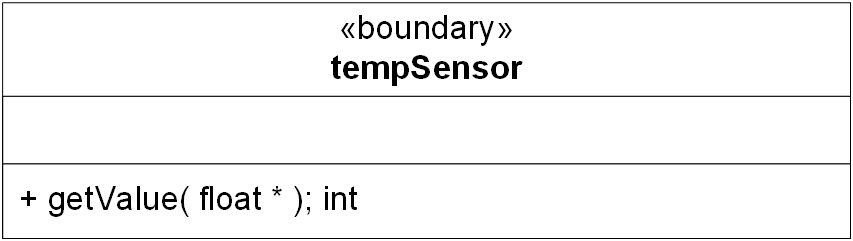
\includegraphics[scale=1.3]{filer/design/Klassediagrammer/sw_psoc_tempSensor}}
\caption{Klasse tempSensor}
\label{fig:sw_psoc_class_tempSensor}
\end{figure} 

{\centering
\textbf{tempSensor}\par
}
\textbf{Ansvar:} Håndterer kommunikationen med temperatursensor. \

\verb+void init( )+ \\
\textbf{Parametre:} Ingen. \\
\textbf{Returværdi:} Ingen. \\
\textbf{Beskrivelse:} Har ingen funktionalitet. \\

\verb+void exit( )+ \\
\textbf{Parametre:} Ingen. \\
\textbf{Returværdi:} Ingen. \\
\textbf{Beskrivelse:} Har ingen funktionalitet. \\

\verb+int getValue( float * )+ \\
\textbf{Parametre:} Pointer til at gemme temperatur i. \\
\textbf{Returværdi:} 0 ved succes ellers negativ i overenstemmelse med fejl-listen. \\
\textbf{Beskrivelse:} Sætter \verb+P_FT2+ benet lavt. Starter A/D-konvertering og omregner modtaget resultat til en temperatur i grader Celsius. \\


\begin{figure}[htbp] \centering
{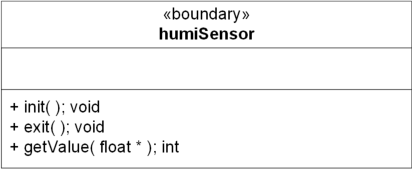
\includegraphics[scale=1.3]{filer/design/Klassediagrammer/sw_psoc_humiSensor}}
\caption{Klasse humiSensor}
\label{fig:sw_psoc_class_humiSensor}
\end{figure} 

{\centering
\textbf{humiSensor}\par
}
\textbf{Ansvar:} Håndterer kommunikationen med fugtighedssensor. \

\verb+void init( )+ \\
\textbf{Parametre:} Ingen. \\
\textbf{Returværdi:} Ingen. \\
\textbf{Beskrivelse:} Har ingen funktionalitet. \\

\verb+void exit( )+ \\
\textbf{Parametre:} Ingen. \\
\textbf{Returværdi:} Ingen. \\
\textbf{Beskrivelse:} Har ingen funktionalitet. \\

\verb+int getValue( float * )+ \\
\textbf{Parametre:} Pointer til at gemme fugtighed i. \\
\textbf{Returværdi:} 0 ved succes ellers negativ i overenstemmelse med fejl-listen. \\
\textbf{Beskrivelse:} Sætter \verb+P_FT2+ benet højt. Starter A/D-konvertering og omregner modtaget resultat til en relativ fugtighed i \%. \\

\begin{figure}[htbp] \centering
{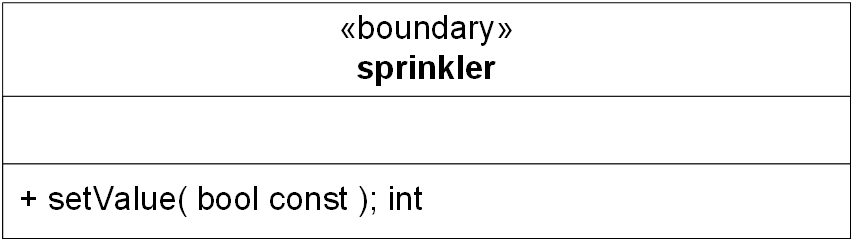
\includegraphics[scale=1.3]{filer/design/Klassediagrammer/sw_psoc_sprinkler}}
\caption{Klasse sprinkler}
\label{fig:sw_psoc_class_sprinkler}
\end{figure} 

{\centering
\textbf{sprinkler}\par
}
\textbf{Ansvar:} At aktivere og deaktivere tilkoblede sprinklere. \

\verb+void init( )+ \\
\textbf{Parametre:} Ingen. \\
\textbf{Returværdi:} Ingen. \\
\textbf{Beskrivelse:} Har ingen funktionalitet. \\

\verb+void exit( )+ \\
\textbf{Parametre:} Ingen. \\
\textbf{Returværdi:} Ingen. \\
\textbf{Beskrivelse:} Har ingen funktionalitet. \\

\verb+int setValue( unsigned char const )+ \\
\textbf{Parametre:} 1 = tænd sprinkler, 0 = sluk sprinkler. \\
\textbf{Returværdi:} 0 ved succes ellers negativ i overenstemmelse med fejl-listen. \\
\textbf{Beskrivelse:} Sætter \verb+PIN+ ud fra modtaget parameter.\\

\begin{figure}[htbp] \centering
{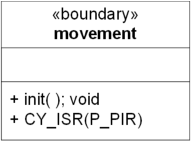
\includegraphics[scale=1.3]{filer/design/Klassediagrammer/sw_psoc_movement}}
\caption{Klasse movement}
\label{fig:sw_psoc_class_movement}
\end{figure} 

{\centering
\textbf{movement}\par
}
\textbf{Ansvar:} Registrere bevægelse fra PIR-sensor. \

\verb+void init( )+ \\
\textbf{Parametre:} Ingen. \\
\textbf{Returværdi:} Ingen. \\
\textbf{Beskrivelse:} Sætter ISR-callback funktion til P\_PIR \\

\verb+CY_ISR(P_PIR)+ \\
\textbf{Parametre:} Ingen. \\
\textbf{Returværdi:} Ingen. \\
\textbf{Beskrivelse:} Kalder \verb+movementDetect()+ i \verb+loadData+-controlleren.\\